\documentclass[dvipsnames,tikz]{standalone}
\usepackage{amsmath}
\usepackage{arevmath}
\usepackage{xcolor}
\usepackage{tikz}
\usetikzlibrary{calc}
\usetikzlibrary{decorations.pathreplacing,calligraphy,3d}
\usepackage{cmbright}      % sansfont

\tikzset{main/.style={draw=black, circle, color=black}}

\begin{document}
	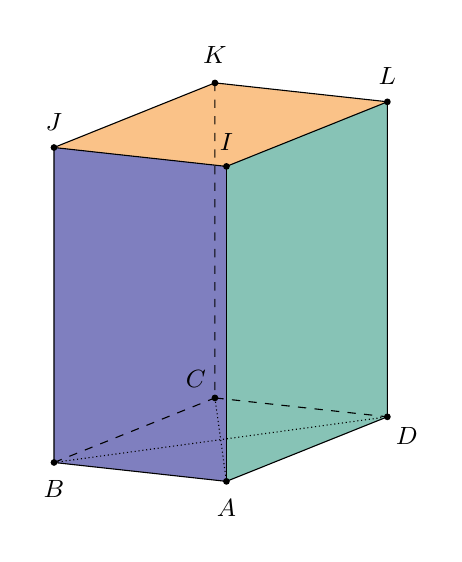
\begin{tikzpicture}[font=\small]
		\fill[BurntOrange, semitransparent] (0,4) -- (2.044,4.820) -- (4.234,4.580) -- (2.19,3.76) -- cycle;
		\fill[PineGreen, semitransparent] (2.19,3.76) -- (4.234,4.580) -- (4.234,0.580) -- (2.19,-0.24) -- cycle;
		\fill[NavyBlue, semitransparent] (0,0) -- (0,4) -- (2.19,3.76) -- (2.19,-0.24) -- cycle;
		\draw [main] (0,4) -- (0,0)-- (2.19,-0.24) -- (4.234,0.580) -- (4.234,4.581) -- (2.044,4.821) -- (0,4) -- (2.19,3.76) -- (4.234,4.580);
		\draw [main] (2.19,-0.24)-- (2.19,3.76);
		
		\draw [main, dashed] (0,0)-- (2.044,0.820);
		\draw [main, dashed] (2.044,4.820) -- (2.044,0.820)-- (4.234,0.580);
		\draw [main, densely dotted] (2.044,0.820)-- (2.19,-0.24);
		\draw [main, densely dotted] (0,0)-- (4.234,0.580);

		\fill[main] (0,0) circle (1pt) node [below] {$B$};
		\fill[main] (2.19,-0.24) circle (1pt) node [below] {$A$};
		\fill[main] (4.234,0.580) circle (1pt) node [below right] {$D$};
		\fill[main] (2.044,0.820) circle (1pt) node [above left] {$C$};
		\fill[main] (0,4) circle (1pt) node [above] {$J$};
		\fill[main] (2.044,4.820) circle (1pt) node [above] {$K$};
		\fill[main] (2.19,3.76) circle (1pt) node [above] {$I$};
		\fill[main] (4.234,4.580) circle (1pt) node [above] {$L$};

	\end{tikzpicture}
\end{document}